\documentclass[11pt,a4paper]{article}
% Presenter's script for the Radiance research showcase poster (13 Oct 2026).
% Build: pdflatex poster_script.tex (twice). House rule for poster material: no em dashes in the text.

\usepackage[margin=2.2cm]{geometry}
\usepackage[T1]{fontenc}
\usepackage{lmodern}
\usepackage{microtype}
\usepackage{amsmath,amssymb}
\usepackage{booktabs}
\usepackage{tabularx}
\usepackage{enumitem}
\usepackage{xcolor}
\usepackage{tikz}
\usetikzlibrary{arrows.meta,positioning}
\usepackage[most]{tcolorbox}
\usepackage[hidelinks]{hyperref}

\definecolor{maroon}{HTML}{7A1712}
\definecolor{slate}{HTML}{3B4556}
\definecolor{soft}{HTML}{F6E9E7}
\definecolor{greyline}{HTML}{A3ABB8}
\definecolor{amber}{HTML}{8A6510}

\setlength{\parindent}{0pt}
\setlength{\parskip}{5pt}
\setlist{itemsep=2pt,topsep=3pt}

% Script blocks
\newtcolorbox{say}[1][]{enhanced,breakable,colback=white,colframe=maroon,boxrule=0.6pt,
  left=8pt,right=8pt,top=5pt,bottom=5pt,arc=2pt,
  title={\small\sffamily\bfseries SAY#1},coltitle=white,colbacktitle=maroon,fonttitle=\sffamily}
\newtcolorbox{key}{enhanced,breakable,colback=soft,colframe=soft,boxrule=0pt,arc=2pt,
  left=8pt,right=8pt,top=5pt,bottom=5pt,
  borderline west={3pt}{0pt}{maroon}}
\newtcolorbox{tech}[1]{enhanced,breakable,colback=white,colframe=greyline,boxrule=0.5pt,arc=2pt,
  left=8pt,right=8pt,top=5pt,bottom=5pt,
  title={\small\sffamily\bfseries #1},coltitle=slate,colbacktitle=slate!8,fonttitle=\sffamily}
\newcommand{\point}[1]{\par\noindent{\sffamily\small\color{slate}\textbf{Point at:} #1}\par}
\newcommand{\keypt}[1]{\begin{key}\sffamily\small\textbf{Key point.} #1\end{key}}
\newcommand{\caution}[1]{\par\noindent{\sffamily\small\color{amber}\textbf{Do not overclaim:} #1}\par}

\begin{document}

\begin{center}
{\sffamily\small\color{maroon}\textbf{TEAM RADIANCE \textperiodcentered{} CSE \textperiodcentered{} UNIVERSITY OF MORATUWA}}\\[6pt]
{\sffamily\LARGE\bfseries Presenting the poster}\\[4pt]
{\sffamily\large Language-Guided Goal Understanding for Simulation-Trained Visuomotor Drone Navigation}\\[8pt]
{\small Speaker script, technical notes and likely questions \textperiodcentered{} 13 October 2026}
\end{center}

\vspace{4pt}
\begin{key}\sffamily\small
\textbf{How to use this.} Section~\ref{sec:pitch} is the one-minute pitch for a passer-by.
Section~\ref{sec:walk} walks the poster panel by panel (about four minutes); read the \textsf{SAY} boxes
aloud in your own words and follow the \textsf{Point at} cues. Section~\ref{sec:deep} holds the technical
detail for examiners: the FiGS pipeline, the lift, FMGS, the query and the evaluation. Section~\ref{sec:nums}
is a one-page numbers sheet and Section~\ref{sec:qa} the likely questions. The QR code on the poster opens
\url{https://radiance-ice-22.github.io/}, which has the recordings of everything shown here.
\end{key}

%──────────────────────────────────────────────────────────────────────────────
\section{The one-minute pitch}\label{sec:pitch}

\begin{say}[ \textperiodcentered{} about 60 seconds]
A drone that flies from camera images alone can be trained entirely in simulation, inside a
photorealistic 3D copy of a real room. That is SOUS VIDE, from Stanford. Its weak point is the training
data: a person places waypoints by hand, and the policy only knows a goal as numbers.

We add meaning to the 3D room. Every one of the half a million Gaussians that make up the scene gets a
feature from two vision models, CLIP and DINOv2. Now you can type a phrase such as \emph{red tool chest}:
the matching Gaussians light up, we pick the object, place a safe approach point in front of it, and an
expert controller flies a course there. No hand-placed waypoints.

We built and evaluated that part: 76\,\% of 29 objects in two rooms are found from the phrase alone, in
under three seconds on a CPU. The next step uses these goals to generate the policy's training data
automatically, and to test whether a policy trained this way handles moving goals and several goals better.
Scan the code to see it working.
\end{say}

%──────────────────────────────────────────────────────────────────────────────
\section{Walking the poster}\label{sec:walk}

\subsection*{01 \textperiodcentered{} The problem \hfill{\normalfont\small 30 s}}
\point{the left column, top.}
\begin{say}
SOUS VIDE's SV-Net is a visuomotor policy: it maps camera images to thrust and body-rate commands at
20\,Hz. It is trained in FiGS, a simulator that renders camera views from a 3D Gaussian splat of a real
room, by imitating an expert controller. But the expert needs a course, and the course is hand-made:
someone places the waypoints. The goal the policy receives is a position, with no idea of \emph{what} it is.
So every new goal needs new hand-made data, each policy learns one trajectory, and results with several
goals are inconsistent.
\end{say}

\subsection*{02 \textperiodcentered{} Aims and hypothesis \hfill{\normalfont\small 30 s}}
\point{the maroon box.}
\begin{say}
We have two aims. First, let scene semantics generate SV-Net's training data automatically: goals are
named in words and found in the 3D scene, and courses and expert flights are generated around them.
Second, develop a language-conditioned visuomotor policy that takes a drone to open-vocabulary target
objects in the trained environment. Our hypothesis is that a policy trained on semantically generated
data does better on dynamic goals, where the same goal moves, and on multi-goal scenarios.
\end{say}
\caution{the hypothesis is not tested yet. Say ``we hypothesise'', never ``we show''.}

\subsection*{03 \textperiodcentered{} Approach \hfill{\normalfont\small 60 s}}
\point{the six boxes across the top; solid boxes 1 to 4, dashed boxes 5 and 6.}
\begin{say}
Six steps. One: capture, a phone video of the room becomes a metric 3D Gaussian splat. Two: add meaning,
we put CLIP and DINOv2 features on every Gaussian. Three: ask, a phrase becomes a 3D goal and a safe
approach point, offline and on a CPU. Four: expert flight, a minimum-snap course to that point, flown by
an MPC expert while FiGS renders what the camera sees. Steps one to four are built and evaluated. Steps
five and six are next: generate many rollouts automatically, with many goals and moving goals, then
train and test SV-Net on them. Note the line underneath: no language model ever runs on the drone. The
language is resolved into a goal before training.
\end{say}
\keypt{Step 2 is where our main technical work sits. We implemented and compared two ways of putting
features on the Gaussians: a training-free \textbf{lift} (LUDVIG / Occam's LGS style) and a trained
\textbf{FMGS} feature field. Section~\ref{sec:deep} explains both.}

\subsection*{The two screenshots (Galley) \hfill{\normalfont\small 30 s}}
\point{the two images under the approach row.}
\begin{say}
This is Galley, the web console we built to run the whole pipeline on the lab GPU. Top: the query
\emph{red tool box} lights up the red tool chest; the green marker is the approach point the drone can
reach, with its 0.19\,m body sphere. Bottom: the course editor, where the goal found for \emph{cart}
becomes the last waypoint of a course the expert flies.
\end{say}

\subsection*{04 \textperiodcentered{} Findings \hfill{\normalfont\small 60 s}}
\point{the bar chart.}
\begin{say}
We evaluated on 29 objects in two rooms, annotated before we looked at any result. The bars are the
top-1 hit rate: did the best candidate land on the right object. Four ways of building the 2D CLIP
features, and for each, two ways of putting them in 3D. Maroon is our training-free lift, grey is the
trained FMGS field. The lift wins for every teacher; the best is 76\,\%, with multi-scale CLIP. FMGS
reaches about half: its matches scatter across the room.
\end{say}
\point{the line chart.}
\begin{say}
Where is the signal lost? We measured the mean relevancy of the right object at three stages: in the
2D teacher, in an ideal crop centred on the object, and in 3D after the lift. For found objects, the 3D
value is within 0.007 of the 2D value. So the lift loses almost nothing; what limits us is the 2D
teacher. For missed objects, the 2D teacher is already below the detection floor of 0.55.
\end{say}
\caution{29 objects is small. No difference between the four teacher designs is statistically
significant, and part of multi-scale's lead comes from its detection floor (Section~\ref{sec:eval}).}

\subsection*{05 \textperiodcentered{} Proposed drone \hfill{\normalfont\small 30 s}}
\point{the CAD render, then the prop-guard chart.}
\begin{say}
This is the airframe we are building to carry the policy: ducted prop guards, 2205 motors, a front
camera, and a Jetson Orin Nano on top to run SV-Net onboard. The prop guard is printed in PA\,12
carbon-fibre nylon. We ran a modal analysis in Fusion: the first natural frequency is 259\,Hz, 30\,\%
above our 200\,Hz target, so the guard does not resonate near the motors' excitation.
\end{say}
\point{the four number tiles.}
\begin{say}
Four numbers: a query takes at most 2.8 seconds on a CPU; refining the camera poses improved the splat by
4.2\,dB; highlighting 532 thousand Gaussians takes 20 milliseconds; and the expert tracks a phrase goal
to within 73\,mm.
\end{say}

\subsection*{06 \textperiodcentered{} Roadmap \hfill{\normalfont\small 20 s}}
\begin{say}
Replicating SOUS VIDE and FiGS is done, and so is phrase to goal to course to expert flight. The
semantic feature fields are partly done: they work, but they need refinement. Next is automatic datasets
and testing SV-Net; the drone build is in progress.
\end{say}

%──────────────────────────────────────────────────────────────────────────────
\section{Technical deep dives}\label{sec:deep}

\subsection{FiGS pipeline: from a phone video to a flying expert}\label{sec:figs}

\begin{center}
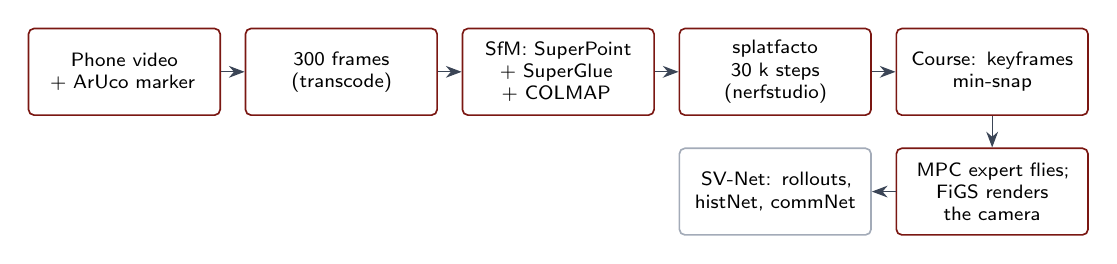
\begin{tikzpicture}[node distance=4mm and 3mm,
  box/.style={draw=maroon,line width=0.6pt,rounded corners=2pt,fill=white,align=center,
    font=\sffamily\scriptsize,minimum height=11mm,text width=22mm},
  arr/.style={-{Stealth[length=2mm]},color=slate}]
\node[box] (v) {Phone video\\+ ArUco marker};
\node[box,right=of v] (f) {300 frames\\(transcode)};
\node[box,right=of f] (s) {SfM: SuperPoint\\+ SuperGlue\\+ COLMAP};
\node[box,right=of s] (t) {splatfacto\\30 k steps\\(nerfstudio)};
\node[box,right=of t] (c) {Course: keyframes\\min-snap};
\node[box,below=of c] (e) {MPC expert flies;\\FiGS renders\\the camera};
\node[box,left=of e,draw=greyline] (r) {SV-Net: rollouts,\\histNet, commNet};
\draw[arr] (v)--(f); \draw[arr] (f)--(s); \draw[arr] (s)--(t); \draw[arr] (t)--(c); \draw[arr] (c)--(e); \draw[arr] (e)--(r);
\end{tikzpicture}
\end{center}

\begin{itemize}
  \item \textbf{Capture.} A phone video of the room with a printed ArUco marker (DICT\_4X4\_50) of known
    size; 300 frames are extracted. The marker fixes the metric scale.
  \item \textbf{Structure from motion.} hloc's SuperPoint features and SuperGlue matches, then COLMAP:
    camera poses (\texttt{transforms.json}, metrically aligned) and a sparse point cloud. Matching is the
    slow stage (about 38 minutes).
  \item \textbf{Splat.} nerfstudio's splatfacto trains the 3D Gaussian splat (30{,}000 steps). Backroom:
    532{,}361 Gaussians, 270 training cameras. Splatfacto also learns a small pose correction per camera;
    using these refined poses renders 4.22\,dB closer to the photos (31.68 vs 27.46\,dB PSNR).
  \item \textbf{Course and expert.} A course is a list of keyframes; FiGS solves a minimum-snap
    trajectory through them, and an MPC expert flies it while FiGS renders the camera image from the splat
    at every step. Our course editor adds a clearance check: drone sphere 0.19\,m, minimum gap 0.15\,m to
    the 5th nearest sparse point.
  \item \textbf{SV-Net (SOUS VIDE's learning half).} The expert flies each course many times with
    randomisation (\texttt{rollout}); a history network (histNet) and a command network (commNet) are
    trained to imitate it from images; \texttt{deploy} flies the student in FiGS. We run these stages
    through Galley's job queue.
\end{itemize}
\keypt{Everything downstream (semantics, courses, flights, training) lives in one frame: the course
frame is the splat frame with $(x, -y, -z)$, so $z$ points down. Goals and annotations are stored in it.}

\subsection{Teachers: the 2D features}\label{sec:teachers}
\begin{itemize}
  \item \textbf{CLIP} (OpenCLIP ViT-B/16, LAION-2B, 512-d), computed LERF-style: crops of several sizes
    slide over each photo, every crop is embedded, giving a feature map per crop scale. The original
    design averaged the scales (FMGS's choice); the default since 8 Oct keeps three scale groups and lets
    each query use the group whose relevancy peaks highest (variant A, \emph{multi-scale}).
  \item \textbf{DINOv2} (384-d) per pixel patch: no language, but sharp object boundaries. Used by FMGS's
    loss and optionally at query time.
  \item Variants we compared: SAM regions (B2: CLIP on segments at three sizes) and a larger CLIP,
    ViT-L/14 (C2).
\end{itemize}

\subsection{The lift: training-free, LUDVIG / Occam's LGS style}\label{sec:lift}
\begin{tech}{What it computes}
Each Gaussian $i$ gets the average of the 2D teacher feature $F_v(p)$ over every training view $v$ and
pixel $p$ it contributes to, weighted by its alpha-blending weight $w_i(v,p)$ at that pixel:
\[
  f_i \;=\; \frac{\sum_{v,p} w_i(v,p)\,F_v(p)}{\sum_{v,p} w_i(v,p)},\qquad
  w_i(p) = \alpha_i(p)\prod_{j<i}\bigl(1-\alpha_j(p)\bigr).
\]
This is the learning-free uplifting of LUDVIG (Marrie et al., 2024) and Occam's LGS (Cheng et al., 2024).
\end{tech}
\begin{itemize}
  \item \textbf{How we compute it.} Rendering is linear in per-Gaussian features, so the numerator is the
    gradient of $\sum_p \langle \mathrm{render}(f), F_v(p)\rangle$ at $f=0$, and the denominator the gradient
    of rendering a constant 1. Two backward passes through gsplat per view; no optimiser, no training. We
    verified these identities on the installed gsplat before using them.
  \item \textbf{A GPU limit we worked around.} gsplat 1.0.0's backward kernel takes at most 32 channels,
    so features go through in 32-channel chunks (CLIP 512 + DINO 384 + weights = 29 passes per image).
  \item \textbf{Cost.} 3 minutes (single-scale) to 18 minutes (multi-scale) on the RTX 2080, under 1\,GB of GPU memory for the lift itself; no training.
  \item \textbf{Refined poses.} The lift uses splatfacto's corrected cameras; with the raw poses features
    land on the wrong Gaussians.
\end{itemize}
\keypt{The lift is not LERF. LERF trains a separate language field; we take LERF's CLIP crop pyramid and
its relevancy score, but put the features into 3D with the LUDVIG / Occam's LGS weighted average.}

\subsection{FMGS: a trained feature field}\label{sec:fmgs}
\begin{tech}{What it is}
FMGS (Foundation Model Embedded Gaussian Splatting) learns a small neural field: a multi-resolution hash
grid (tiny-cuda-nn) evaluated at each Gaussian's centre, with two heads that output a CLIP (512-d) and a
DINOv2 (384-d) feature. Features are rendered through the frozen splat and trained to match the teacher
maps.
\end{tech}
\begin{itemize}
  \item \textbf{Our implementation.} A standalone trainer (not an \texttt{ns-train} plugin). The splat is
    frozen (its checksum is identical before and after); the most opaque 40\,\% of Gaussians are trained;
    features rendered at 480\,$\times$\,270.
  \item \textbf{Loss.} $\;\mathcal{L} = 0.2\,\mathrm{Huber}(\text{CLIP}) + 0.8\,\lVert\text{DINO}\rVert_2^2
    + 0.01\,\text{pixel alignment}$; Adam, learning rate $10^{-2}\!\to\!10^{-3}$, 4{,}200 steps.
  \item \textbf{Cost.} 31.4 minutes and 7.95\,GB of the 8\,GB card.
  \item \textbf{Problems we solved.} On the RTX 2080 (sm\_75) a 192-d hash grid fails to launch, so the 24
    levels run as two 12-level grids of 8 features (levels within 1\,\% of FMGS's; a reported deviation).
    The CLIP gradients underflowed in fp16 until we added dynamic loss scaling; memory fragmentation was
    fixed with PyTorch's expandable segments.
  \item \textbf{Why it loses to the lift.} Its misses are mostly ``no candidate'': high-relevancy Gaussians
    scattered across the room instead of one cluster on the object. The lift averages exactly what each
    Gaussian was seen as, so it has no such smoothing artefacts.
\end{itemize}

\subsection{From a phrase to a goal}\label{sec:query}
\begin{enumerate}
  \item \textbf{Relevancy (LERF).} With cosine similarities $s_q$ to the phrase and $s_{n_j}$ to the
    canonical negatives \emph{object, things, stuff, texture}, and temperature $T=10$:
    \[ \mathrm{rel}_i = \min_j \; \sigma\bigl(T\,(s_q - s_{n_j})\bigr). \]
  \item \textbf{Relative threshold.} $\tau = 0.55 + 0.5\,(\text{peak} - 0.55)$, where the peak is the mean
    of the top 100 relevancies. A fixed 0.55 let every white surface into ``whiteboard''.
  \item \textbf{Clusters.} Selected Gaussians are grouped by voxel connected components (0.1\,m); each
    cluster is scored by $\sum(\mathrm{rel}-\tau)\cdot\text{opacity}$. The best one is the goal.
  \item \textbf{Approach point.} 1.0\,m from the goal, towards the cameras that saw it, kept inside the
    flyable box; its clearance is checked against the drone's 0.19\,m sphere.
  \item The query runs on a CPU worker: about 0.7\,s with single-scale tables and 2 to 2.8\,s with the
    multi-scale default.
\end{enumerate}

\subsection{How we evaluated}\label{sec:eval}
\begin{itemize}
  \item \textbf{Frozen sets.} 29 objects present (13 backroom, 16 flightroom) and 6 absent objects,
    annotated before any result was seen. The five early backroom queries that shaped the threshold are a
    separate development set.
  \item \textbf{Hit rule.} The top candidate's box (plus 0.3\,m) contains an annotated instance, or its
    centre is within 0.75\,m of one.
  \item \textbf{Results (CLIP query).} Lift: single-scale 20, multi-scale 22, SAM regions 21, ViT-L/14 19
    of 29. FMGS: 15, 15, 12, 10.
  \item \textbf{The floor effect.} Multi-scale takes the best of three scale groups, which raises every
    peak by about 0.045, including for absent objects. Compared at an equal number of absent objects
    firing (2 of 6), SAM regions without level choice find 24, single-scale 23, multi-scale 22. Those floors
    were read off the evaluation set, so they are optimistic and post hoc.
\end{itemize}
\keypt{Safe claims: the training-free lift beats the trained field for every teacher; lifting loses almost
nothing; the bottleneck is the 2D teacher. Unsafe claim: ``multi-scale is the best design''.}

\subsection{SV-Net status}
The first student cohort (p4\_smoke: backroom, circuit course) runs through all SV-Net stages in 49
minutes, but the student does not fly the course yet: the expert tracks to 1.7\,cm, the student's mean
tracking error is 9.4\,m. The next cohort uses a larger dataset. The hypothesis test waits on a student
that flies.

\subsection{Prop guard modal analysis}
Autodesk Fusion, PropGuard v9, PA\,12 carbon-fibre nylon (EOS PA 603-CF), 8 modes, 32{,}849 parabolic
elements, fixed at two mounts. Modes 1 to 4: 259.0, 266.6, 285.8 and 294.7\,Hz; highest computed 501.4\,Hz.
The first mode is 30\,\% above the 200\,Hz design target.

%──────────────────────────────────────────────────────────────────────────────
\section{Numbers sheet}\label{sec:nums}
\begin{center}\small
\begin{tabularx}{\linewidth}{@{}lX@{}}
\toprule
Scene & backroom, 532{,}361 Gaussians, 270 training cameras (300 frames) \\
Pose refinement & +4.22\,dB PSNR (31.68 vs 27.46\,dB) \\
Top-1, lift (CLIP query) & 69 / 76 / 72 / 66\,\% (single-scale / multi-scale / SAM / ViT-L) \\
Top-1, FMGS & 52 / 52 / 41 / 34\,\% \\
Relevancy per stage & found 0.682 $\to$ 0.748 $\to$ 0.675; missed 0.485 $\to$ 0.577 $\to$ 0.517; floor 0.55 \\
Query time & about 0.7\,s single-scale, at most 2.8\,s multi-scale, CPU only \\
Recolouring & 532\,k Gaussians in 20\,ms (+71\,ms for the next frame) \\
Expert tracking to a phrase goal & at most 73\,mm (browser gate); 8\,mm (automated gate) \\
FMGS training & 4{,}200 steps, 31.4\,min, 7.95\,GB on an RTX 2080 \\
Lift & 3 to 18\,min, under 1\,GB, no training \\
Drone & 33\,$\times$\,29\,$\times$\,10\,cm, 2205 motors, Jetson Orin Nano, body sphere 0.19\,m \\
Prop guard & first mode 259\,Hz (target 200\,Hz) \\
SV-Net student & expert 1.7\,cm, student 9.4\,m mean tracking error: not flying yet \\
\bottomrule
\end{tabularx}
\end{center}

%──────────────────────────────────────────────────────────────────────────────
\clearpage
\section{Likely questions}\label{sec:qa}

\newcommand{\qa}[2]{\par\smallskip\noindent{\sffamily\bfseries\color{maroon} Q. #1}\par\noindent #2\par}

\qa{Is the lift LERF?}{No. LERF trains a language field. Our lift is the training-free weighted average
of LUDVIG and Occam's LGS. We use LERF's CLIP crop pyramid and its relevancy score with canonical negatives.}

\qa{Why does a training-free method beat a trained one?}{The lift gives each Gaussian exactly the average of
what it looked like in the photos. FMGS has to fit a smooth field with limited capacity, and on our scenes
its high-relevancy points scatter across the room, so the clustering finds no clean object.}

\qa{Does a language model run on the drone?}{No. The phrase is resolved into a 3D goal offline, before
training. The drone only runs SV-Net.}

\qa{Is the policy language-conditioned today?}{Not yet. Today language picks the goal and builds the course.
Aim 2, a policy that takes open-vocabulary targets, is the next stage of the project.}

\qa{What happens when the object is not in the room?}{If nothing clears the threshold, no goal is made. On
the website, ``bicycle'' returns nothing. Two of six absent objects still fire; we think at least one is a
real look-alike in the room, and that set is being re-checked.}

\qa{Are 29 objects enough?}{Enough to show the large effects (lift vs FMGS, 2D vs 3D), not to rank the four
teacher designs: those differences are not statistically significant.}

\qa{Why Gaussian splatting?}{It renders photorealistic camera views fast enough to train a visuomotor policy
in simulation (that is FiGS), and its explicit Gaussians give us something to attach meaning to.}

\qa{Why does the student not fly yet?}{The first cohort was a small smoke test. The pipeline runs end to end;
the next cohort uses a larger dataset. We report the 9.4\,m error rather than hide it.}

\qa{How do you keep the drone safe near the object?}{The approach point is 1\,m from the goal, inside the
flyable box, and its gap to the scenery is checked against the 0.19\,m body sphere with a 0.15\,m margin.
The course editor flags any path that comes closer.}

\qa{What did you build yourselves?}{The install and pipeline automation for FiGS and SOUS VIDE; Galley,
the web console; the whole semantics package (teachers, lift, FMGS trainer, query, evaluation); and the
drone design. SOUS VIDE and FiGS are Stanford MSL's.}

\end{document}
